\chapter{Testy środowiska symulacyjnego}
\label{sec:tests}
W tym rozdziale przedstawione są różne konfiguracje pakietów, wraz z wykresami ruchów platform, oraz wnioski płynące z tych zachowań.
Każdy test wymaga innego podłączenia pakietów do siebie nawzajem.

Uruchomiono odpowiednią konfigurację pakietów i połączono je strumieniami konfiguracyjnymi.
Wiadomości przesyłane w odpowiednich strumieniach zostały zapisane do pliku za pomocą narzędzia
\texttt{rosbag}, dostępnego w środowisku ROS.
Za pomocą narzędzia \texttt{rostopic}, wyeksportowano dane z plików do pliku rekordów, gdzie każde pole oddzielone jest przecinkiem (\emph{Comma Separated Value}(CSV)).
Używając skryptu w programie Gnuplot, narysowano wykresy w formacie PDF, które następnie załączono poniżej.

\section{Weryfikacja działania modelu dynamiki}
	W tym teście porównano działanie modelu dynamiki oraz jej enkoderów w stosunku do zadanego sterowania.
	W tym celu uruchomiono scenę posiadającą dwa modele kinematyki i jeden dynamiki oraz obserwator symulacji, patrz rysunek \ref{uml:comparison}.
	Jeden model kinematyki użyto do przekształcania zadanych prędkości kół do prędkości liniowej i kątowej platformy, którą to za pomocą symulatora scałkowano w celu określenia zadanej trasy robota. Drugi model, korzystając z enkoderów, realizował mechanikę odometrii, wyznaczał trasę na podstawie danych o obrotach kół.
	Wiadomości, zawierające dane ich pozycje w czasie, były zapisywane do pliku.
	Dodatkowo, wtyczka symulatora, obserwator symulacji, generowała dane porównujące odległość i kąt obrotu modeli od siebie.
	
	\begin{figure}[h]
		\centering
		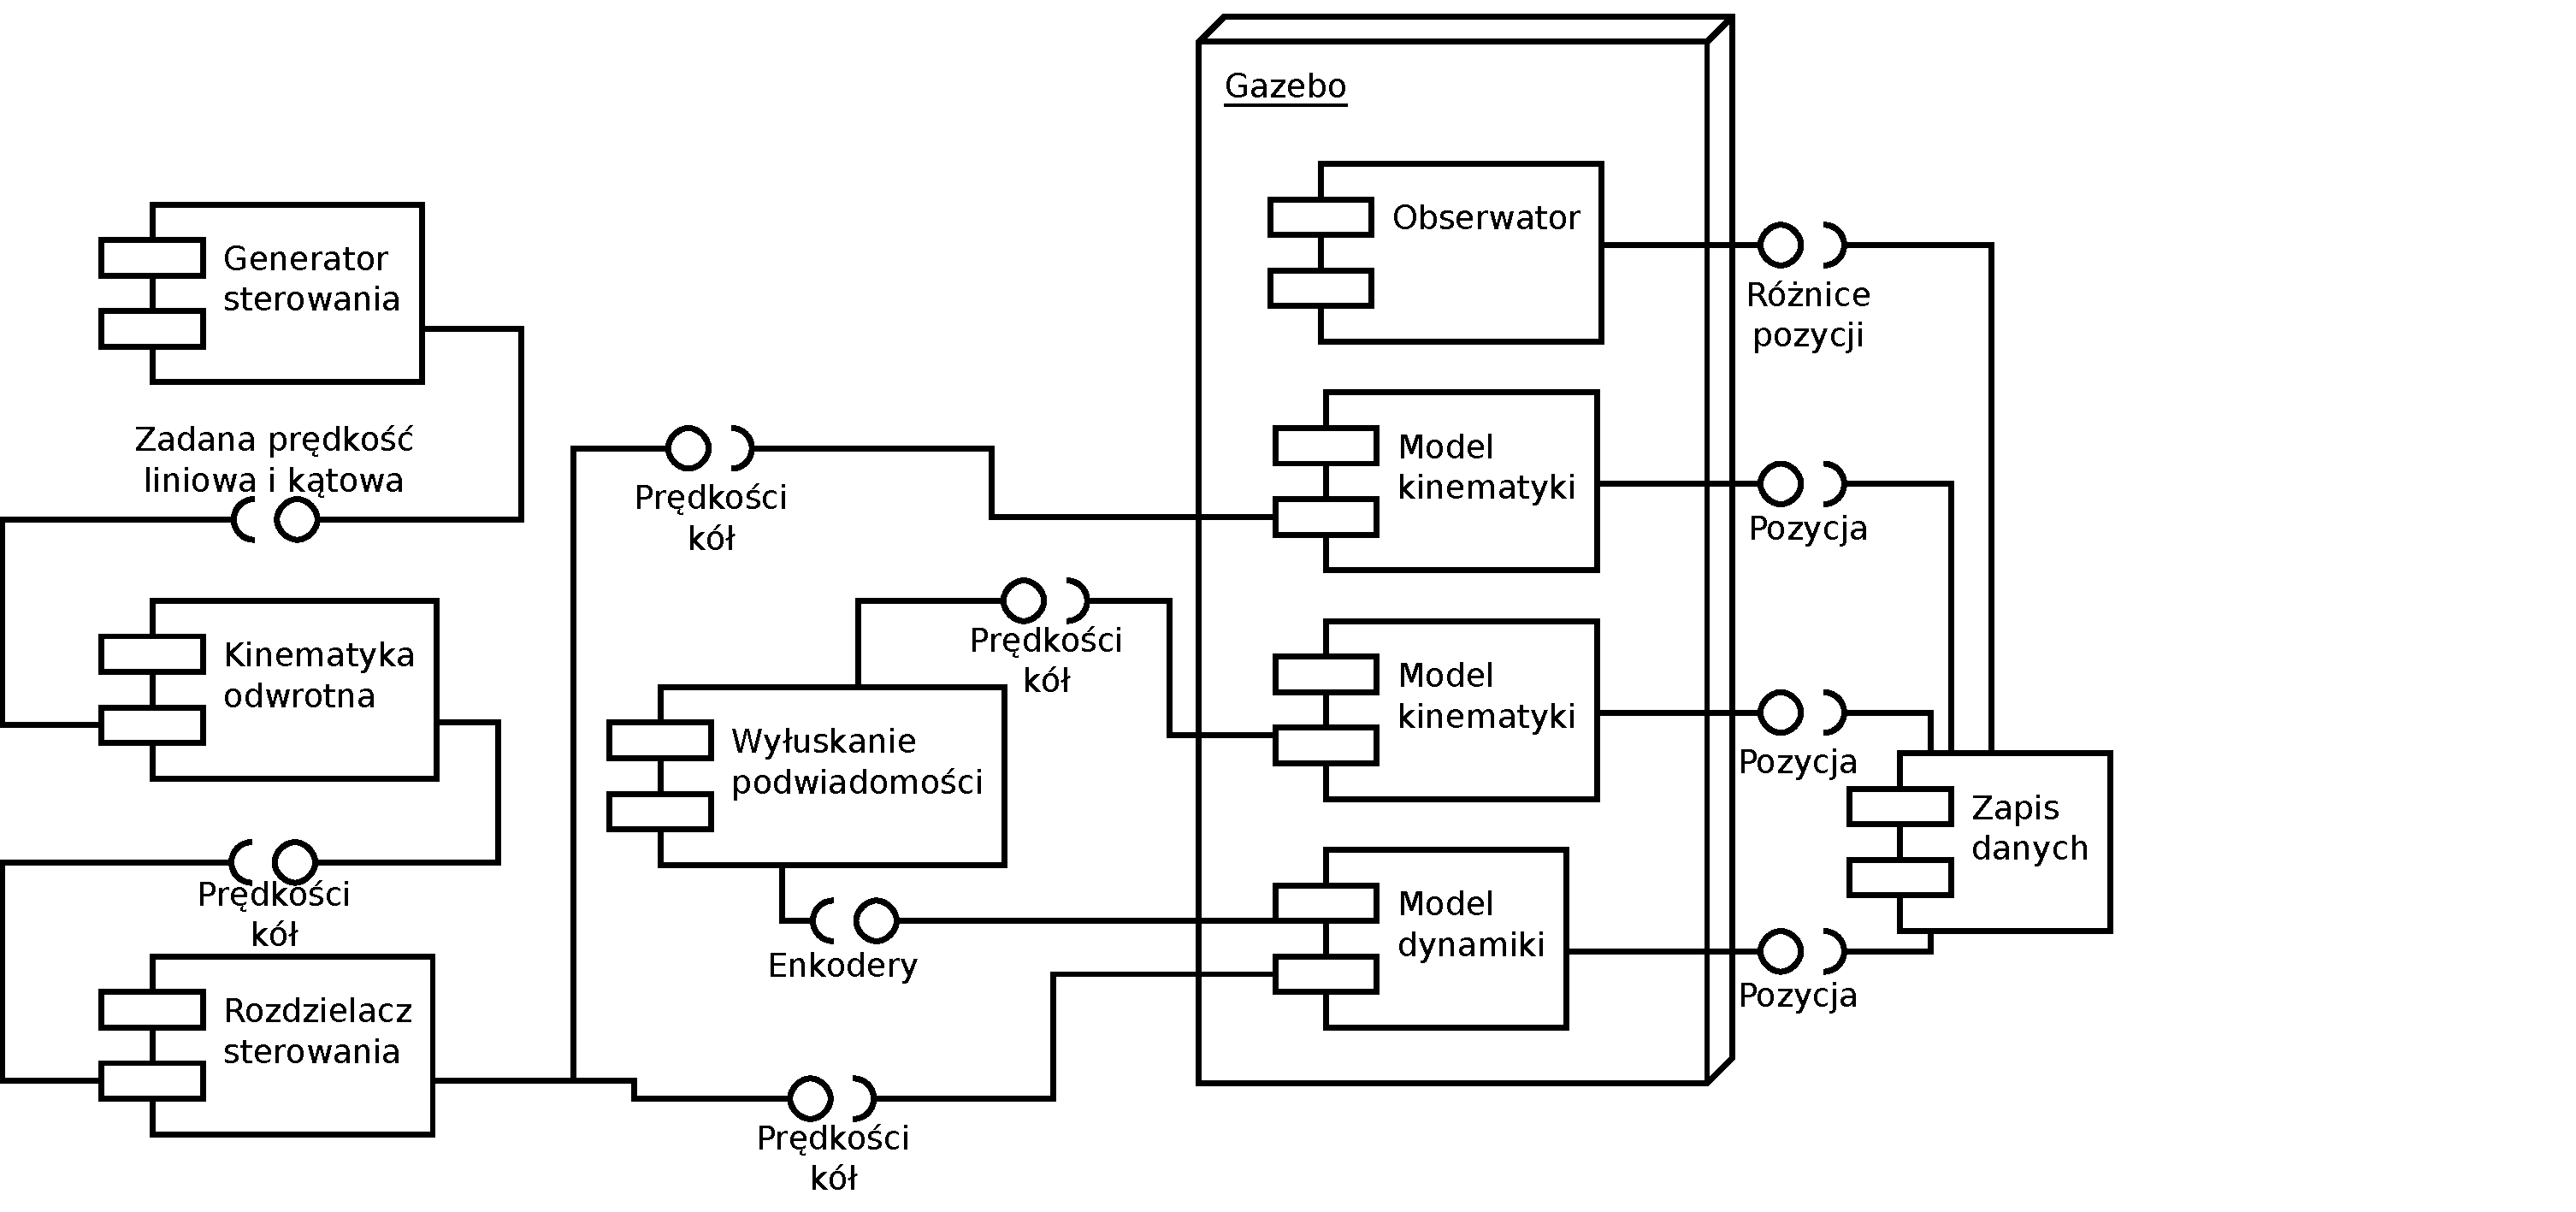
\includegraphics[width=\textwidth]{uml/comparison.pdf}
			\caption{Połączenie pakietów w teście porównującym modele.}
		\label{uml:comparison}
	\end{figure}
	
	\subsection{Porównanie modeli}
		Za pomocą pakietu do nadawania sterowania, opisanego w sekcji \ref{sec:gramofon}, nadano trasę o kształcie przedstawionym na rysunku \ref{plot:comparison_xy}.
		W tym teście robot kolejno poruszał się:
		\begin{enumerate}
			\item W przód z prędkością 0,25 \si{\metre\per\second} przez 5 \si{\second}.
			\item W prawo z prędkością $\pi/32$ \si{\metre\per\second} oraz prędkością kątową o $\pi/32$ \si{\radian\per\second} wokół osi Z, przez 8 \si{\second}.
			\item W tył z tą samą prędkością i przez ten sam czas, jak w punkcie 1.
			\item W prawo z prędkością $\pi/16$ \si{\metre\per\second} oraz prędkością kątową $\pi/32$ \si{\radian\per\second} wokół osi Z, przez 8 \si{\second}.
		\end{enumerate}
		Powyższe akcje wykonał czterokrotnie.
		
		\begin{figure}[H]
			\centering
			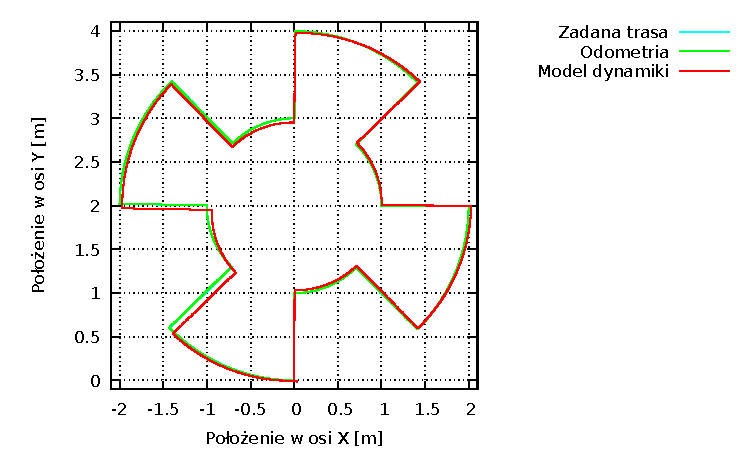
\includegraphics[width=\textwidth]{plots/comparison_xy.pdf}
				\caption{Trasa modelu platformy w teście porównującym modele. Różnica między zadaną trasą, a trasą wyznaczoną przez enkodery, jest niewielka.}
			\label{plot:comparison_xy}
		\end{figure}
		
		\begin{figure}[H]
			\centering
			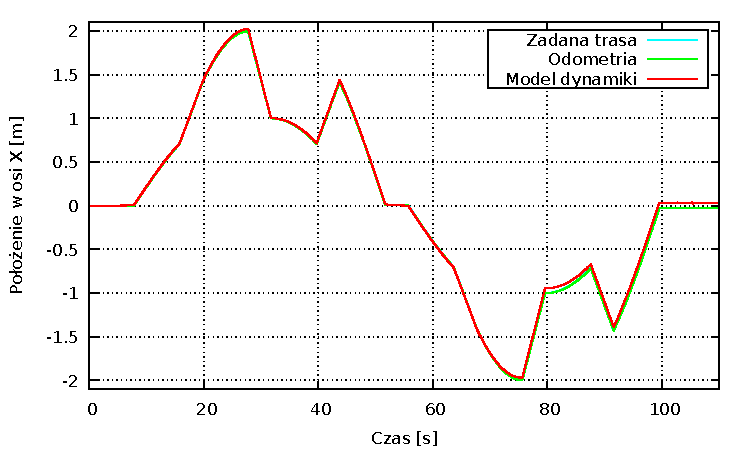
\includegraphics[width=\textwidth]{plots/comparison_xt.pdf}
				\caption{Składowa pozycji modelu wzdłuż osi X w czasie.}
			\label{plot:comparison_xt}
		\end{figure}
		
		\begin{figure}[H]
			\centering
			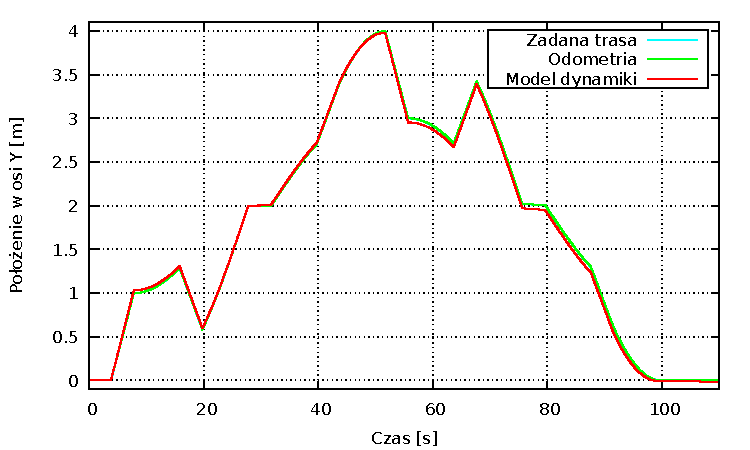
\includegraphics[width=\textwidth]{plots/comparison_yt.pdf}
				\caption{Składowa pozycji modelu wzdłuż osi Y w czasie.}
			\label{plot:comparison_yt}
		\end{figure}
		
		\subsubsection{Dokładność odometrii}
			Trasa obliczana na podstawie obrotu kół byłaby identyczna do zadanej trasy w przypadku gdyby koła obracałyby się dokładnie z zadanymi prędkościami.
			To wymagałoby, aby silniki kół posiadały nieskończony moment obrotowy, lub na tyle duży, aby opór obrotu, spowodowany tarciem, nie wpływał 
			znacząco na ich prędkość kątową. Innymi słowy, nawet jeśli platforma uderzyłaby w przeszkodę, koła nadal powinny obracać się zgodnie z zadanymi wartościami.
			To nie oznacza, że rzeczywista trasa robota jest zgodna z obliczoną z odometrii, gdyż uwzględnia także poślizgi kół, czego enkodery nie są w stanie wykryć.
			
			Różnice w pozycji zadanej, a pozycji obliczonej za pomocą danych wygenerowanych przez enkodery biorą się z tego, że
			silniki mogą nie mieć wystarczającej mocy, aby nadać kołom odpowiednie prędkości i przeciwdziałać oporom.
			Ponieważ założono dużą moc silników, jak zostało to opisane w sekcji \ref{sec:encoders}, modelowane koła są mniej podatne na opory, a co za tym idzie, 
			ich prędkość będzie bardziej zbliżona do prędkości zadanej i także trasa wyznaczona w ten sposób z odometrii będzie niemalże pokrywać się z zadaną trasą.
			
			Zauważalne różnice pomiędzy przebiegami trasy odometrycznej i zadanej pojawiają się przy wywoływaniu dużych przyspieszeń i poślizgów na modelu platformy.
			
		\subsubsection{Trasa modelu dynamiki}
			Różnica pomiędzy położeniem modelu dynamiki, a kinematyki (położenia zgodnego z zadaną trasą), rośnie w czasie.
			Jest tak na skutek błędów numerycznych maszyny do symulacji fizyki, braku systemu operacyjnego czasu rzeczywistego, braku wszystkich oporów i skomplikowanej budowy modelu.
			Ten model także uwzględnia współczynniki tarcia kół o podłoże i jest w stanie modelować ich poślizgi.
			
			\begin{figure}[H]
				\centering
				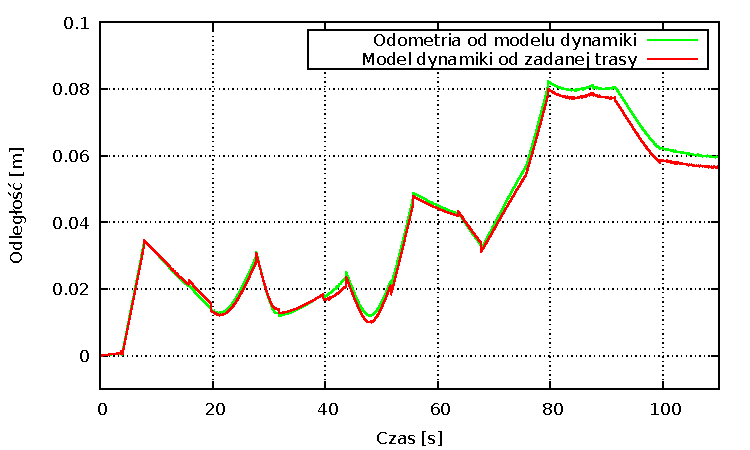
\includegraphics[width=\textwidth]{plots/comparison_dt.pdf}
					\caption{Różnica pomiędzy położeniem modelu dynamiki i modelem kinematyki modelującym zadaną pozycję i pozycję odometryczną.}
				\label{plot:comparison_dt}
			\end{figure}
			
			\begin{figure}[h]
				\centering
				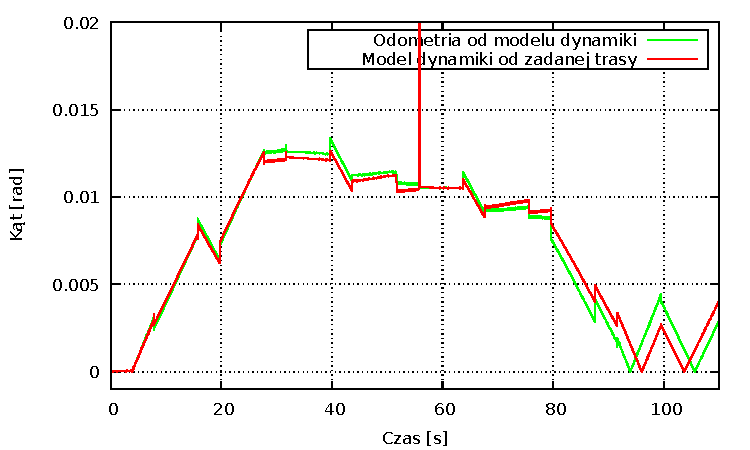
\includegraphics[width=\textwidth]{plots/comparison_at.pdf}
					\caption{Różnica pomiędzy orientacją modelu dynamiki i modelem kinematyki modelującym zadaną pozycję i pozycję odometryczną.}
				\label{plot:comparison_at}
			\end{figure}
			
		\subsubsection{Zachowanie modelu dynamiki}
			Na wykresie \ref{plot:comparison_dt} zamieszczono różnice między pozycjami odpowiednich modeli.
			Różnice nie zmieniają się monotonicznie ze względu na zmiany kierunków prędkości robota i jego obrót wokół osi Z.
			Dlatego też, zdarzają się przypadki w których model dynamiki zbliża się do modelu kinematyki (zadanej pozycji) po tym gdy oddalił się od niej już wcześniej.
			
			Oba wykresy zmieniają się w podobny sposób, gdyż na obie różnice wpływają poślizgi kół w trakcie trasy, jednak wykres odometrii jest podatny na te poślizgi.
			Różnice pomiędzy wykresami powstają na skutek modelowania tarcia kół o podłoże. 
			Enkodery są wstanie wykryć zwiększone tarcie kół na skutek obliczenia różnicy zadanego obrotu a faktycznego.
			Takie tarcie towarzyszy nagłym zmianom prędkości platformy, lecz to nie powoduje że są w stanie wykryć poślizg.
			Inaczej mówiąc, przyspieszenia platformy powodują trudności w obrocie kołami na skutek tarcia i możliwe poślizgi, lecz enkodery są w stanie wykryć i obliczyć tylko różnice w obrocie, co nie powoduje możliwości wykrycia poślizgów.
			
			Przykładowe różnice pomiędzy wykresami występują na przykład w 15 sekundzie ruchu. 
			W tym miejscu nastąpił nagły zwrot bazy, który spowodował tarcie, a co za tym idzie i zwiększony opór ruchu obrotowego kół.
			Ten opór został wykryty przez enkodery, lecz poślizg nadal wpłynął na pozycję modelu dynamiki w większym stopniu.
			Dlatego też różnica między pozycją odometryczną, a pozycją modelu dynamiki wzrosła mniej, niż różnica pomiędzy pozycją modelu dynamiki, a pozycją wynikającą z zadanej trasy.
			
			Na wykresie \ref{plot:comparison_at} są pokazane różnice pomiędzy kątem obrotu wokół osi Z tych modeli.
			Podobnie, jak w przypadku położenia, enkodery są w stanie wykryć część zmian kierunku ruchu platformy.
			Na zmianę różnicy kąta obrotu nie wpływają jedynie zmiany prędkości kątowej, a również losowy kąt obrotu nadany platformie w przypadku poślizgów.
			Można zauważyć, że różnica między orientacją modelu dynamiki, a orientacją wyliczoną na podstawie odometrii zwykle zmienia się mniej dynamicznie od 
			różnicy między modelem dynamiki, a zadaną pozycją.
			
	\subsection{Powtarzalność testów}
		Zadano modelowi jazdę z różnymi prędkościami po trasie kwadratu, wyznaczona trasa została przedstawiona na rysunku \ref{plot:repetitions_xy}.
		
		\begin{figure}[h]
			\centering
			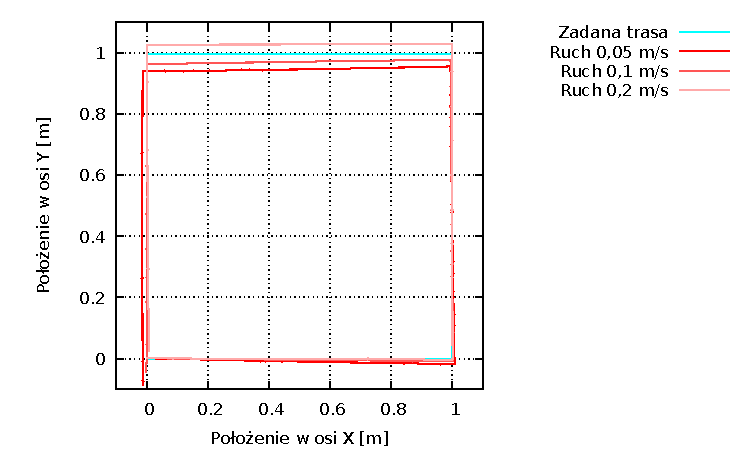
\includegraphics[width=\textwidth]{plots/repetitions_xy.pdf}
				\caption{Trasa modeli platformy, poruszających się z różną prędkością liniową po trasie kwadratu. W tym eksperymencie nie nadano prędkości kątowej.}
			\label{plot:repetitions_xy}
		\end{figure}
		
		Eksperyment pokazuje, że zależnie od prędkości przejazdu, mogą występować niedokładności ruchu. Dzieje się to głównie w kierunku Y, gdyż ruch
		platformy w bok jest zawsze podobny. Im wolniej platforma się porusza, tym mniejszą odległość pokonuje w odpowiednio dłuższym czasie. 
		 %TODO Dlaczego?
		 
\section{Porównanie modelu z robotem}
	Za pomocą generatora sterowania, zadano platformie ruch po trasie kwadratu w prędkością 0,1 \si{\metre\per\second}.
	Zapisano dane generowane przez enkodery, obliczaną odometrię, pomiary skanerów laserowych oraz samo sterowanie.
	Następnie, używając tych samych danych, przeprowadzono identyczny eksperyment na modelu, łącząc pakiety w sposób pokazany na rysunku \ref{uml:comparison}.
	Korzystając z pakietu \texttt{laser\_scan\_matcher}, obliczono rzeczywistą pozycję platformy, korzystając z danych skanerów laserowych.
	Określenie pozycji jest obarczone błędem, wynikającym
	z błędów pomiarowych czujników, stąd obliczona trasa nie składa się z odcinków i posiada szum.
	Trasy modeli i platformy pokazano na wykresie \ref{plot:velmobil_xy}.
	
	\begin{figure}[h]
		\centering
		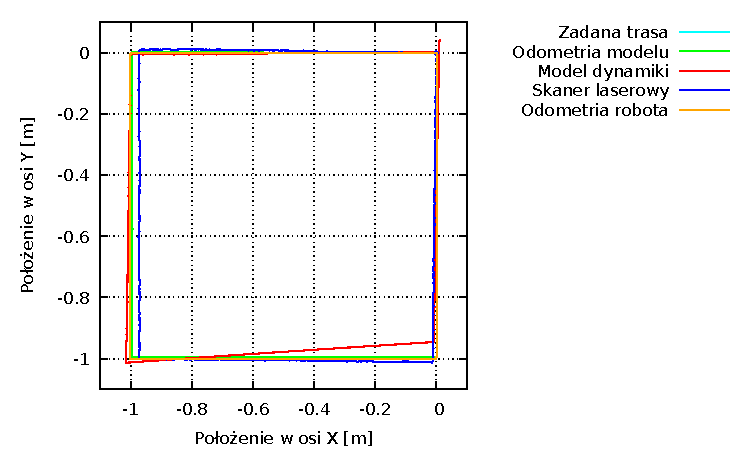
\includegraphics[width=\textwidth]{plots/velmobil_xy.pdf}
			\caption{Trasa modeli robota przy jeździe po trasie kwadratu.}
		\label{plot:velmobil_xy}
	\end{figure}
	
	Charakterystyczną cechą wykresu jest to, że robot przejechał mniejszą odległość wzdłuż osi X, niż wzdłuż osi Y.
	Może być to spowodowane różnicą w wyjściowym współczynniku tarcia kół w zależności od wyjściowego wektora prędkości kół.
	Zgodnie z cechą kół, opisaną w sekcji \ref{sec:robot_movement}, rolki kół obracają się z największą prędkością przy ruchu w bok, a co za tym idzie, w ruchu ma udział także
	ich tarcie obrotowe. Przy ruchu w przód, rolki nie obracają się, więc i to dodatkowe tarcie nie wpływa na ruch platformy.
	Dlatego też platforma pokonała mniejszą odległość w jednym z kierunków.d
	
	%TODO dlaczego enkodery tego nie wykryły?
	
	
	
	
	
		
% \section{Jednostka inercyjna}
% \label{sec:test_imu}
% 	\begin{figure}[H]
% 		\centering
% 		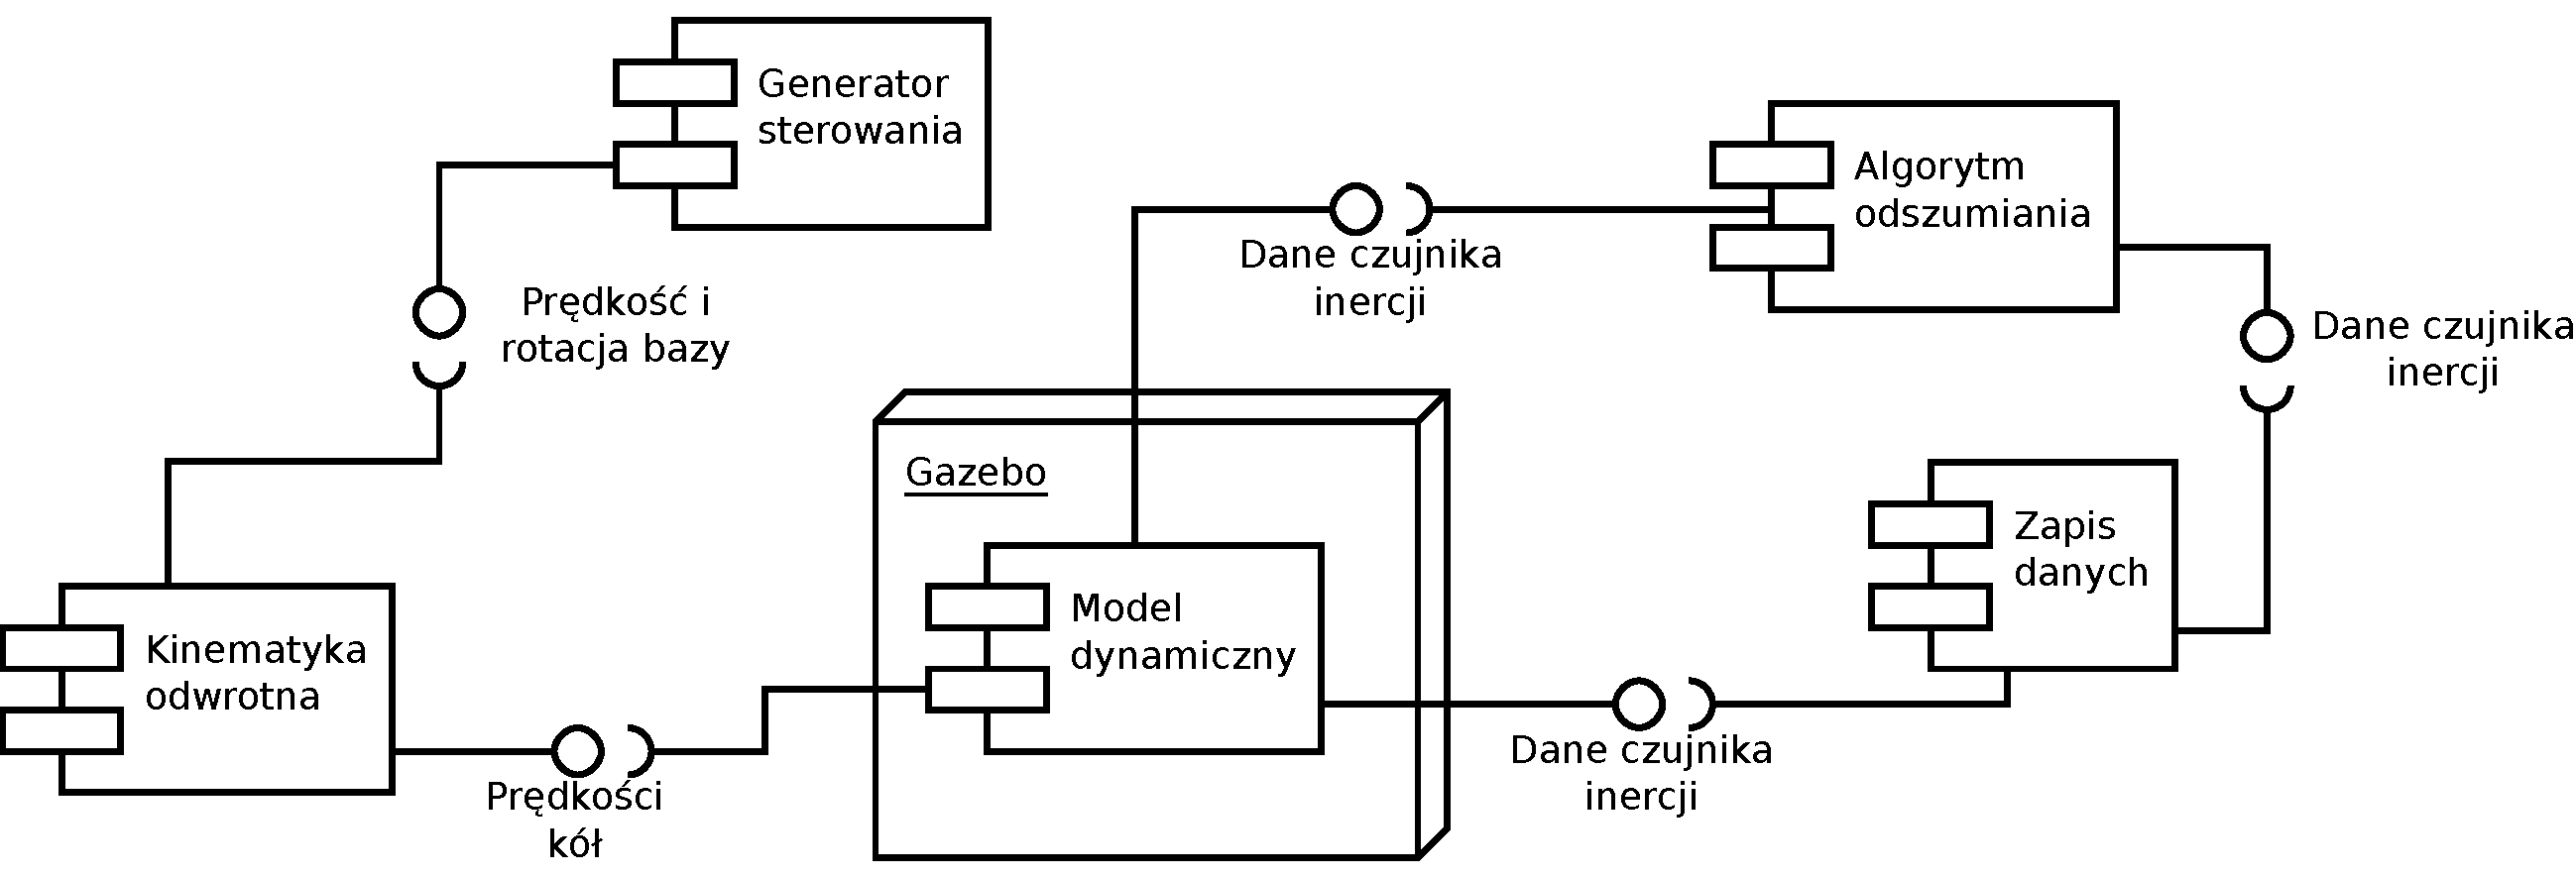
\includegraphics[width=\textwidth]{uml/wewucho.pdf}
% 		\caption{Połączenie pakietów dla testu jednostki inercyjnej.}
% 		\label{uml:test_imu}
% 	\end{figure}
% 	\subsection{Akcelerometr}
% 		Dane zostały zebrane w trakcie testu \ref{sec:test_pose}.
% 		Połączenie pakietów w sposób pokazany na rysunku \ref{uml:test_imu}.
% 		Dane wygenerowane przez ten czujnik są obarczone bardzo dużym błędem.
% 		
% 		\begin{figure}[H]
% 			\centering
% 			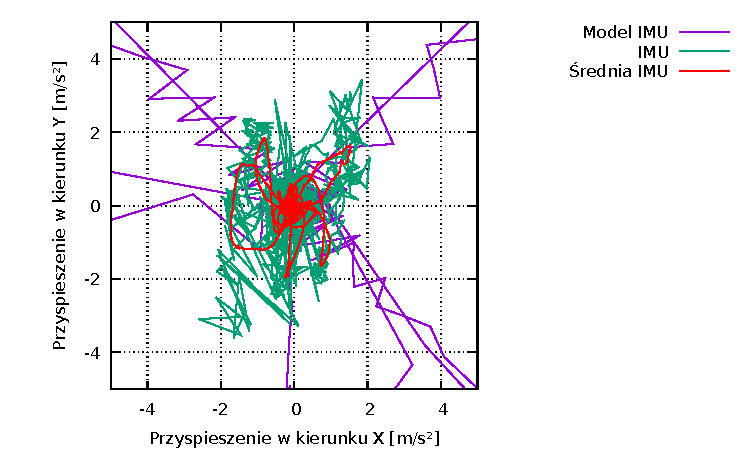
\includegraphics[width=\textwidth]{plots/wewucho.pdf}
% 			\caption{Odczyt akcelerometra z jednostki inercyjnej i jej modelu.}
% 			\label{plot:imu}
% 		\end{figure}
% 		
% 		\subsubsection{Impulsy na wykresie modelu}
% 			W trakcie testu następowały kolejne przyspieszenia i opóźnienia bazy w zadanych kierunkach, to widać jako impulsy na wykresie.
% 			Na początku platforma zaczęła poruszać się w kierunku -X i w tą stronę zostało nadane pierwsze przyspieszenie.
% 			Nie jest znana jego wielkość, gdyż było to wysłanie jednej wiadomości, bez płynnego narastania prędkości.
% 			
% 			Następnie zadziałało przyspieszenie zmieniające prędkość liniową platformy o 90°, co oznacza że impuls jest obrócony o 45° względem układu współrzędnych.
% 			Impuls wystąpił w kierunku (X,-Y). 
% 			
% 			Podobna zmiana prędkości nastąpiła jeszcze dwa razy, generując kolejne, symetryczne impulsy.
% 			
% 			Platforma zatrzymała się, generując opóźnienie w kierunku -Y, co także widać na wykresie.
% 			
% 			Przeprowadzanie podobnych testów pokazuje, że nawet jeśli ustawić zaplanowane przyspieszenie modelu, to i tak czujnik nie zwraca poprawnych amplitud.
% 			Jedyne, co wiadomo to to, że generuje proporcjonalnie większe wartości dla większych przyspieszeń.
% 			Również istnieje korelacja pomiędzy osiami, na przykład natychmiastowe zatrzymanie się w jednym z kierunków powoduje inne przyspieszenie, niż w innym kierunku.
% 			Co zresztą jest logiczne, gdyż osie kół stawiają większy opór, gdy działający na nie moment siły jest skierowany prostopadle do osi, niż równolegle. 
% 			Zatem większe opóźnienie będzie przy hamowaniu z jazdy w bok, niż jazdy w przód.
% 			
% 			Szum spowodowany jest potrzebą różniczkowania prędkości obliczanej dyskretnie. Wartości mas i momentów inercji ogniw modelu mocno wpływają na kształt, kolerację
% 			osi i szum na wykresie. Nie jest technologicznie możliwe zamodelować doskonałej jednostki inercyjnej ze względu na błędy numeryczne, algorytmy użyte w maszynie
% 			symulującej fizykę i system operacyjny na którym pracuje symulator.
% 			
% 		\subsubsection{Wykres czujnika}
% 			Porównując te dwa wykresy razem, nie widać zależności, jednak zastosowanie prostego uśrednienia pakietem opisanym w sekcji \ref{sec:odszumiacz} powoduje, że impulsy wygenerowane przez robota również są widoczne. Każda uśredniona wartość jest średnią z 40 poprzednich.
% 			
% 			Można zaobserwować jak każdy impuls ma kształt półksiężyca, na początku każdej zmiany prędkości opóźnienie ma kierunek równoległy do wektora prędkości, zatrzymując robota, następnie wolniejsze przyspieszenie
% 			nadaje nowy kierunek, a potem następuje reakcja korpusu i gasnące drgania w nowym kierunku. Zamodelowanie tej własności mogłoby okazać się bardzo trudne, prawdopodobnie należałoby nadać dodatkowe ogniwa do robota i połączyć je więzami sprężynowymi.
% 			
% 			Aby użyć tego czujnika do obliczania pozycji, trzeba wpierw użyć zaawansowanego algorytmu odszumiającego i wyprowadzić eksperymentalnie zależności pomiędzy czujnikami
% 			osi (macierz kowariancji).
% 			Dopiero wtedy można wprowadzić dodatkowy szum do modelu jednostki inercyjnej w celu przybliżenia jej wyjścia do rzeczywistego urządzenia.
% 
% 			
% \subsection{Żyroskop}
% 		\label{sec:test_ang}
% 		Czujnik prędkości kątowej korzysta z żyroskopu i zwraca prędkość kątową we wszystkich trzech osiach.
% 		Ponieważ jednak platforma porusza się po płaskim terenie, wymagany jest jedynie czujnik mierzący obrót wokół osi Z, czyli w górę.
% 		Drugą osią wykresu może być zatem czas nadania pakietu. Te dane zostały zebrane w trakcie testu \ref{sec:test_pose}.
% 		
% 		\begin{figure}[H]
% 			\centering
% 			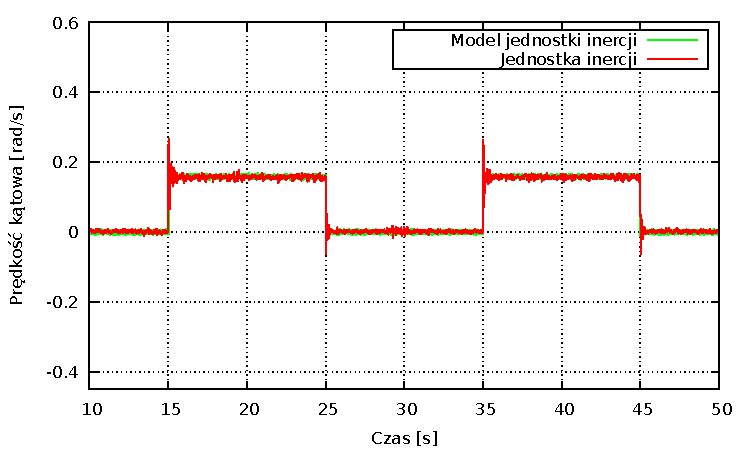
\includegraphics[width=\textwidth]{plots/wewucho_ang.pdf}
% 			\caption{Odczyt żyroskopu z jednostki inercyjnej i jej modelu.}
% 			\label{plot:ang}
% 		\end{figure}
% 		
% 		Ponieważ maszyna do symulacji fizyki wewnętrznie posiada informację o prędkościach obiektów, model tego czujnika po prostu zwraca gotowe dane. 
% 		To powoduje, że praktycznie pozbawiony jest szumu. 
% 		Aby zatem polepszyć jakość symulacji, dodano sztuczny szum do generowanych danych, zgodnie z tabelą \ref{tab:imu_noise}.
% 		W ten sposób wykresy są do siebie bardziej zbliżone.
% 		
% 		Jednak niektórych własności czujnika nie da się zamodelować tak łatwo. Po pierwsze, szum czujnika nie do końca ma rozkład normalny.
% 		Z wykresu można zobaczyć, że dane prawdopodobnie korelują z częstotliwościami obrotu kół.
% 		Dodatkowo, nagła zmiana prędkości kątowej powoduje zauważalny skok na wykresie, co w symulatorze jest znacznie mniej widoczne.
% 		Ta cecha wykresu zależy od ustawień mas i inercji ogniw modelu, lecz z kolei inne ustawienia inercji powodują większe błędy przy poruszaniu się platformy.
% 		
% 		
% 		
% 	
% 	

%TODO różnica współczynników tracia w bok i do przodu
